%%%%%%%%%%%%%%%%%%%%%%%%%%%%%%%%%%%%%%%%%%%%%%%%%%%%%%%%%%
%
% Západočeská univerzita v Plzni
% Fakulta aplikovaných věd
% Katedra informatiky a výpočetní techniky
%
%%%%%%%%%%%%%%%%%%%%%%%%%%%%%%%%%%%%%%%%%%%%%%%%%%%%%%%%%%

\documentclass[czech,BP]{thesiskiv}

% Definujte údaje pro vstupní strany

\author{Jakub Váverka}
\declarationmale

% Název práce
\title{Generátor a parser formulářů recenzí příspěvků na konferenci TSD}

% 
% Texty abstraktů (anglicky, česky)
%
\abstracttexten{
Generator and Parser of Submission Review Forms for the TSD Conference

Goal of this work is the creation of a modul for web page of TSD conference. On this web page there are located member submissions. This modul allows downloading of a rating form, to which can user fill in his review. User can later upload his review into the TSD system. In the theoretical part of this work, I focus on technologies, that allow manipulation with form files. Later I focus on the creation of form itself and it's possible modifications. This thesis also contains documentation of this module. The last part contains results of my testing.}

\abstracttextcz{Cílem této práce je vytvoření modulu pro webové stránky konference TSD. Na těchto stránkách se nacházejí články členů konference. Tento modul umožní stažení hodnotícího formuláře, do kterého bude možné vyplnit recenze těchto článků. Následně bude možné jednotlivé recenzi nahrát do systému a uložit vyplněná data. V teoretické části této práce se zabývám technologiemi, které umožňují práci s těmito formuláři. Poté se věnuji samotnému průběhu tvorby formuláře a jeho možnému rozšíření. Součástí této práce je i dokumentace modulu. Na závěr komentuji výsledky testování.
}

%%%%%%%%%%%%%%%%%%%%%%%%%%%%%%%%%%%%%%%%%%%%%%%%%%%%%%%%%%
%
% DODATEČNÉ BALÍČKY PRO SAZBU
%
%%%%%%%%%%%%%%%%%%%%%%%%%%%%%%%%%%%%%%%%%%%%%%%%%%%%%%%%%%
\usepackage{eurosym}
% Zařadit literaturu do obsahu
\usepackage[nottoc,notlot,notlof]{tocbibind}
\usepackage{listings}
\lstset{frame=tb,
  language=php,
  aboveskip=3mm,
  belowskip=3mm,
  showstringspaces=false,
  columns=flexible,
  basicstyle={\small\ttfamily},
  numbers=left,
  breaklines=true,
  breakatwhitespace=true,
  tabsize=3
}
% Umožňuje vkládání obrázků
\usepackage[pdftex]{graphicx}

% Odkazy v PDF jsou aktivní; navíc se automaticky vkládá
% balíček 'url', který umožňuje např. dělení slov
% uvnitř URL
\usepackage[pdftex]{hyperref}
\hypersetup{colorlinks=true,
  unicode=true,
  linkcolor=black,
  citecolor=black,
  urlcolor=black,
  bookmarksopen=true}

% Při používání citačního stylu csplainnatkiv
% (odvozen z csplainnat, http://repo.or.cz/w/csplainnat.git)
% lze snadno modifikovat vzhled citací v textu
\usepackage[numbers,sort&compress]{natbib}

%%%%%%%%%%%%%%%%%%%%%%%%%%%%%%%%%%%%%%%%%%%%%%%%%%%%%%%%%%
%
% VLASTNÍ TEXT PRÁCE
%
%%%%%%%%%%%%%%%%%%%%%%%%%%%%%%%%%%%%%%%%%%%%%%%%%%%%%%%%%%
\begin{document}
%
\maketitle
\tableofcontents

\chapter{Úvod}
Cílem této práce je navrhnout a implementovat rozšíření již stávajícího webového portálu pro konferenci TSD. Text, Speech and Dialogue, dále jen TSD, je konference, která probíhá každoročně. Setkání se koná každé září a umístění se střídá mezi Brnem a Plzní. Obě umístění mají pro TSD zřízený vlastní webový portál a můj modul bude součástí toho plzeňského.

Tato konference se zabývá například rozpoznáváním, pochopením, generováním a obecně interakcí lidského jazyka s~počítačem. Uživatelé mohou každoročně přihlásit své články do systému. Tyto články jsou později ohodnoceny členy programového výboru, a buď schváleny nebo odmítnuty. Vyplnění tohoto hodnocení probíhalo doposud jen skrze online formulář. Některým uživatelům však trvalo vyplnění recenze příliš dlouho. Pokud není formulář odeslán do určité doby, dojde ke ztrátě vyplněných dat.

Mým úkolem je navrhnout způsob jak vyplňování formuláře uživatelům co nejvíce zpříjemnit a umožnit jim hodnocení těchto článků i bez přístupu k internetu. Zároveň musí být řešení dostatečně jednoduché, jelikož se nedá počítat s~vysokou počítačovou zdatností uživatelů. Pro uživatele by bylo ideální, pokud by mohl jednoduše stáhnout jediný soubor, který by obsahoval článek, který má hodnotit a bylo by i možné hodnocení rovnou vyplnit.

Pokud bych zvolil formát souboru, který je pro takové věci určený, bude pravděpodobně neznámý a musel bych po uživatelích požadovat instalaci dodatečných programů. Pokud bych naopak zvolil formát otevíratelný v textovém editoru, zmátl bych nezkušené uživatele a umožnil bych jim zničit strukturu potřebnou k zpětnému zjištění dat. Ideální se zdá být využití formátu PDF. Tento formát je sice velmi rozšířený, ale poměrně uzavřený. Navíc se tento formát nepoužívá jen na textové soubory, a tak není snadno editovatelný. To bude představovat výzvu pro implementaci.

\section{Textové formáty}
Z průzkumu jsem zjistil, že získání odpovědí na různé dotazníky a vyplňování formulářů, se v dnešní době realizuje hlavně pomocí textových formátů. V praxi je totiž pořád rychlejší vytvořit dokument v programu \emph{Microsoft Word} nebo \emph{Microsoft Excel}, rozeslat ho a poté ručně hodnoty zadat do systému. Tento postup však není možný u větších systémů, jakým je webový portál TSD. Je nutné tento postup zautomatizovat. Problém je v tom, že textové soubory může uživatel kompletně změnit. Vytvoření programu, který by byl schopen takové soubory načítat, je obtížné. Proto se budu nejprve snažit využít formátů, které jsou pro vyplňování formulářů určené. 
\section{Adobe}
Adobe Systems Incorporated je společnost, která byla založena Johnem Warnockem a Charlesem Geschkem  v roce 1980. Zakladatelé byli do té doby součástí výzkumného týmu ve společnosti Xerox. Jejich prvním produktem byl software nazývaný PostScript. PostScript je programovací jazyk, který dokáže tiskárně popsat rozvržení stránky. Toto byl v té době velký pokrok, který jim vydělal velké množství peněz. Firma Adobe na tento úspěch navázala mnoha dalšími produkty, mezi které patří například první volně škálovatelný font, program na tvorbu maleb Adobe Illustrator a mimo jiné i Portable Document Format neboli PDF\cite{Adobe_story}. 

PDF jako formát pro sdílení a tisknutí elektronických souborů byl zveřejněn v roce 1993. Velmi rychle rozdrtil konkurenci a stal se standardem, který každý zná a běžně využívá každý den. PDF se postupně vyvíjelo. Z první verze 1.0 je již momentálně verze 1.7 a touto nejnovější verzí se stalo PDF standardem ISO. 

Adobe vydalo program pojmenovaný \emph{Acrobat Reader}, který slouží ke čtení tohoto formátu. Tento program byl nejdříve placený, ale v současné době je zdarma a tvoří výbavu skoro každého počítače. To je jeden z důvodů, proč je právě tento formát ideální pro mou práci\cite{Adobe_history}.
Přestože Adobe umožňuje uživatelům zdarma používat software na čtení tohoto formátu, již neumožňuje tento formát zdarma editovat či jinak měnit. K takovým operacím slouží program s~názvem \emph{Adobe Acrobat}. Licence na tento program musí být placena měsíčně. Navíc je \emph{Adobe Acrobat} určen především pro klasické uživatele, kteří budou pracovat skrze grafické rozhraní. Tímto programem není možné vytvořit dokument použitím příkazové řádky nebo nějakým automatizovaným způsobem. 

\subsection{Formuláře}
Formát PDF může obsahovat i dynamický obsah, v podobě vyplnitelných formulářů. Bezplatná verze programu Acrobat Reader však neumožňuje tvorbu takových souborů. K tvorbě formulářů uživatel potřebuje plnou placenou verzi Adobe Acrobat. Po vytvoření takového souboru jej může samozřejmě sdílet s~jinými uživateli, kteří ji mohou vyplnit i bezplatnou verzí Acrobat Reader \cite{Adobe_forms}. 
Formuláře firmy Adobe jsou uzavřená záležitost. 

Samotnou realizaci formuláře lze provést několika způsoby. Během vývoje PDF formulářů firma Adobe používala více technologií. Většina těchto technologií využívala servery k získání odpovědí od uživatelů. Tyto servery již byly odstaveny, takže se dané technologie dají využít jen ve velmi omezené míře. Tyto systémy nejsou vytvořeny tak, aby bylo snadné automaticky nahrávat odpovědi do databáze. Adobe předpokládá, že bude autor formulářů odpovědi od uživatelů sbírat pomocí grafického programu \emph{Acrobat Reader} a dále je konvertovat třeba do tabulek \emph{Excel}. 

Adobe se snaží tyto technologie navrhovat pro podnikatele a obchodníky. K jejich využití tedy uživatel nepotřebuje skoro žádné počítačové znalosti. Prvním programem na tvorbu formulářů od Adobe byl \emph{Acrobat Forms Data Format Toolkit}, který má bezplatnou licenci.
\subsection{Acrobat FDF Toolkit}
FDF neboli Forms Data Format je formát navržený firmou Adobe. Slouží k uložení dat vyplněných do formuláře v souboru PDF. Uživatel vyplní formulář a pak místo uložení celého souboru, uloží odděleně soubor s~koncovkou \emph{fdf}, který obsahuje pouze identifikátory polí a uživatelův vstup. Tento malý soubor může uživatel odeslat na server, kde je díky znalosti souboru PDF, ze kterého byl soubor FDF vytvořen, možné zjistit, co uživatel vyplnil. K největší úspoře dochází ve chvíli, kdy je soubor PDF velký, protože nemusíme zbytečně odesílat celý jeho obsah na server, ale stačí jen malý soubor s~odpověďmi. Adobe se navíc pokusilo tímto formátem do jisté míry přiblížit webovým formulářům. 

Firma Adobe umožňuje zakoupení a instalaci serverového softwaru, který přijímá přes internet FDF soubory od uživatelů, kteří formulář vyplnili. Uživateli se v \emph{Adobe Readeru} objeví možnost odeslání formuláře. Tento způsob se zdá velmi chytrý. Adobe od něj však upustilo a je udržován spíše kvůli zpětné kompatibilitě. Jsem přesvědčen o tom, že většina uživatelů o této vlastnosti PDF formulářů neví a jednou z důležitých vlastností, které by mělo mé řešení splňovat je intuitivnost, proto jsem od tohoto řešení upustil.

\subsection{Acrobat LiveCycle Designer}
Dalším vývojovým stádiem Adobe formulářů byl \emph{LiveCycle Designer}. Cílem tohoto programu bylo vytvořit PDF soubory, které uvnitř obsahují text ve formátu XML. Tyto formuláře se nazývají XFA forms. Designer umožňuje rozšířit schopnosti takových souborů přidáním funkčního kódu v jazyce JavaScript nebo skriptovacího jazyka FormCalc, který navrhlo samotné Adobe.

Formuláře vytvořené pomocí \emph{LiveCycle Designer} však nejsou kompatibilní s~jinými programy od firmy Adobe. Mohou být samozřejmě vyplněny, ale ne již změněny. \emph{LiveCycle Designer} byl součástí programu Adobe Acrobat až do verze X. 

Po této verzi se Adobe rozhodlo prodávat \emph{LiveCycle Designer} jako samostatný produkt. To způsobilo mnoho nepříjemností uživatelům, kteří o této změně nevěděli a aktualizovali svůj Adobe Acrobat z verze X na verzi XI, protože jim byl během instalace \emph{LiveCycle Designer} odinstalován. Adobe neumožňuje verzi programu, downgradovat a to znamenalo, že tito uživatelé již nemohli své formuláře nijak upravovat, dokud si od firmy Adobe nezakoupili i samostatnou licenci na \emph{LiveCycle Designer}. To samozřejmě vzbudilo vlnu odporu, a tak Adobe začalo umožňovat jednorázové získání licence \emph{LiveCycle Designer} pro uživatele, kteří zakoupili produkt Adobe Acrobat před datem 15. října 2012 \cite{Adobe_LVD}\cite{Adobe_LVD_forum}.
\subsection{FormsCentral}
\emph{FormsCentral} byl poslední pokus Adobe k ovládnutí trhu s~online formuláři. Tento program se, jako i oba předchozí, soustředil na možnost vyplnění PDF formuláře přímo na webu a použití externích serverů na ukládání odpovědí. Při vytvoření firma Adobe očekávala, že bude o takovou službu mnohem větší zájem, než který ve skutečnosti vznikl. Adobe však pomocí \emph{FormsCentral} nenabídlo uživatelům takové změny, kvůli kterým by stálo na novou platformu přejít. Nezájem způsobil to, že byla i tato služba ukončena 28. července 2015. Ještě před ukončením se na trhu objevilo více dalších služeb, které nabízí naprosto stejné vlastnosti a dokonce umožňují i naimportovat již stávající tabulky z \emph{FormsCentral}\cite{Adobe_FormsCentral}.

\subsection{Alternativy FormsCentral třetích stran}
Samotná firma Adobe na svých stránkách, které se zabývají přerušením služby \emph{FormsCentral} doporučuje, aby uživatele přešli na jednu z alternativ. Nejpopulárnější podle nich jsou \emph{Formstack}, \emph{JotForm}, \emph{Survey Monkey} a \emph{WuFoo}. Některé z těchto služeb umožňují hostování serveru na ukládání odpovědí zdarma, do určitého limitu počtu uložených odpovědí \cite{Adobe_FormsCentral}. 
Pro tuto práci ale není ideální, aby byla závislá na službách třetí strany, které by mohly postupem času skončit. Navíc se tyto služby soustředí na vyplňování formulářů online, a to je již realizováno na webových stránkách TSD pomocí webového formuláře. Hlavním cílem této práce je navrhnout formuláře, které lze vyplnit i bez připojení k internetu a následně je možné je přes webové stránky pouze nahrát. Proto se nebudu ve své práci těmito webovými servery nadále zabývat.

\section{PDFLib}
\emph{PDFlib} je jeden z nejrozšířenějších a nejúspěšnějších nástrojů na vytváření a úpravu souborů ve formátu PDF. Jeho hlavním cílem je tvorba dynamických souborů, které obsahují data z databáze, pomocí webového serveru nebo libovolných serverových systémů. Je realizován jako knihovna pro PHP. Povedlo se jí zjednodušit práci se soubory PDF, a tak umožňuje, aby se programátor soustředil na skládání komponent na stránku, místo procházení komplikovaného formátu PDF. Knihovna PDFlib je na trhu již od roku 1997 a nabízí velký sortiment různých balíčků. Tato knihovna je placená. Nejlevnější je základní verze pro osobní počítač, která v současné době stojí \euro 375. Pokud chce však uživatel využít tuto knihovnu na strojích IBM nebo Oracle, zaplatí za licenci až \euro 3990, a to jen za základní verzi, která se soustředí především na vytváření souborů. 

Firma \emph{PDFlib GmbH}, která tuto knihovnu poskytuje, nabízí i další zajímavé služby. Patří mezi ně například knihovna PDI, která se soustředí na importování. Umožňuje tedy vzít již existující PDF dokument a přidat do něj další stránky. Také umožňuje přidat záhlaví a zápatí nebo vložit vodoznak a jinou grafiku. Tato knihovna samozřejmě již nedokáže měnit stávající obsah nebo interagovat s~dynamických obsahem. A to jsou právě vlastnosti, které jsou pro nás důležité. 

Další knihovna této firmy se nazývá \emph{TET}, což je zkratka pro Text and Image Extraction Toolkit. Jak již název naznačuje, tato knihovna se zabývá extrakcí textu, obrázků a metadat ze souborů formátu PDF. Obrázky jsou uloženy v běžných grafických formátech, zatímco texty tato knihovna ukládá jako speciální XML soubory, kterým se říká \emph{TETML}. \emph{TET} toho docílí za pomoci analytických algoritmů, které zjišťují umístění a formátování textu. 

Poslední knihovna od firmy \mbox{\emph{PDFlib GmbH}}, která stojí za zmínku, se jmenuje PLOP a zabývá se linearizací, optimalizací a ochranou PDF souborů. Linearizace vizuálně urychluje stažení PDF souboru, klientovi se nejdříve odešlou nejdůležitější informace a PDF se tedy zobrazí v kratším čase, než kdyby bylo odesláno klasickým způsobem. Uživatel tedy může prohlížet dokument dříve, než má stažená všechna data. Zbytek dat se stáhne na pozadí. Optimalizace je u PDF velmi užitečná, protože dva stejné PDF soubory mohou mít naprosto rozdílné velikosti. PLOP dokáže takové soubory projít a smazat veškeré redundantní informace. Tím docílí menší velikosti souborů, aniž by snížil kvalitu. Co se zabezpečení týče, mohou mít PDF soubory nastaveny zámky například na tisk nebo extrakci dat. Tento nástroj dokáže zámky odemknout a daný obsah zpřístupnit. Uživatel musí samozřejmě znát heslo nebo vlastnit certifikát, jímž byl dokument uzavřen. PLOP dokáže navíc i projít poškozenou PDF strukturu a pokusit se ji opravit. S~těmito dalšími knihovnami samozřejmě stoupá i cena licence. Firma PDFlib GmbH sice umožňuje stažení omezené verze PDFlib Lite 7, ale tato verze je spíše demonstrace toho, co dokáže plná verze. Navíc firma ukončila vývoj a PDFlib Lite 7 není od roku 2010 udržován\cite{PDFlib}.

Knihovna je psaná v jazyce C, lze ji však použít v mnoha jazycích. Mezi ty nejznámější patří ANSI C, ANSI C++, Java, .NET, Perl, Python a PHP. Samozřejmě je potřeba před použitím knihovnu různě upravit nebo obalit, to je však již přehledně popsáno v dokumentaci\cite{PDFlib_Manual}.

  
\section{FPDF}
\emph{FPDF} je třída určená pro programovací jazyk PHP. Umožňuje generování PDF souborů pomocí čistého PHP, to znamená bez použití knihovny \emph{PDFlib}, která je psaná v jazyce C. F v názvu znamená "free". Tato třída je dostupná naprosto zdarma a může být využívána a upravována podle jakýkoliv potřeb. Knihovna \emph{FPDF} je lehčí verzí knihovny \emph{TCPDF}, obě zvládají podobné věci, ale TCPDF má více funkcí. Dokáže například interpretovat HTML. Protože je knihovna \emph{TCPDF} postavena na knihovně \emph{FPDF}, syntax kódu pro generování stránek se moc neliší \cite{FPDF}\cite{FPDF_Book}. 
\subsection{FPDI}
\emph{FPDI} je kolekce PHP tříd, které umožňují vývojářům číst stránky z již existujícího PDF dokumentu. Její využití je také zdarma. Ke svému běhu potřebuje knihovnu \emph{FPDF}\cite{FPDI}.
\section{mPDF}
Knihovna \emph{mPDF} je rozšíření předchozí knihovny \emph{FPDF}. Především se soustředí na generování PDF souborů z HTML. Na rozdíl od svého předchůdce dokáže tato knihovna již použít kódování UTF-8. \emph{mPDF} také dokáže aplikovat na dodané HTML kaskádové styly, a tak se přiblížit vzhledu, který by HTML kód měl, pokud by byl zobrazen v internetovém prohlížeči. Tyto vlastnoti jsou vykoupeny větší velikostí souborů a delším časem, který je potřeba pro generování souborů. \cite{mPDF}
\section{DOMPDF}
\emph{DOMPDF} se velmi podobná knihovně \emph{mPDF}, ale na rozdíl od \emph{mPDF}, která vychází z \emph{FPDF}, tato knihovna potřebuje ke své funkci nainstalovaný nástroj \emph{PDFlib}. Pokud uživatel tento nástroj nemá, může využít pro vytváření dokumentů přiloženou třídu \emph{R\&OS CPDF}. Generování dokumentů za pomoci této třídy je pomalejší a více paměťově náročné, ale je tím zaručeno, že \emph{DOMPDF} nebude závislá na žádné externí knihovně. Jelikož není v dokumentaci této knihovny žádná zmínka o kódování, předpokládám, že neumí kódovat UTF-8, proto považuji předchozí knihovnu za lepší volbu a k \emph{DOMPDF} bych se uchýlil jen ve chvíli, kdy by \emph{mPDF} nedokázalo vykreslit obsah podle mých představ.  \cite{DOMPDF}
\section{Snappy}
Další způsob generování PDF souborů v programovacím jazyce PHP je obalová knihovna \emph{Snappy}. Tato knihovna umožňuje snadné využití konzolové aplikace \emph{wkhtmltoPDF}. Nástroj \emph{wkhtmltoPDF}, jak již název napovídá, se využívá k převádění HTML na PDF. Knihovna \emph{Snappy} jej tedy obaluje, aby bylo možno tento nástroj snadno použít i v jazyce PHP. Programu stačí předat URL a výstupem je soubor, který vypadá identicky jako stránka, která se na daném URL nachází\cite{Snappy}\cite{wkhtmltoPDF}.
\section{TCPDF}
\emph{TCPDF} je třída v jazyce PHP určena ke generování PDF dokumentů a dodnes je nejpoužívanější. Je to hlavně díky tomu, že je využívána v mnoha populárních PHP aplikacích. \emph{TCPDF} původně vznikla jako odnož třídy \emph{FPDF}, ale postupem času přibylo množství funkcí a dnes je skoro kompletně přepsána. Díky tomu, že je tak bohatě využívána, vzniklo na internetu velké množství návodů a příkladů, které budou při vývoji aplikací, které tuto třídu využívají, velmi užitečné. 

\emph{TCPDF} ke generování PDF dokumentů nepotřebuje žádné externí knihovny. Automaticky vytváří dokumenty ve správných formátech a následně umožňuje si tyto formáty libovolně přizpůsobit a definovat například vlastní okraje nebo jednotky měření. 

Třída \emph{TCPDF} zvládá generovat dokumenty v kódování UTF-8. Součástí této třídy jsou i nástroje pro zpětné importování existujících PDF dokumentů. Bohužel jsou stále ve vývoji a nemusíme jejich použitím dojít ke kýženým výsledkům. \cite{TCPDF} \cite{FPDF_Book}
\section{PDF Parser}
Pokud bychom chtěli importovat již existující PDF dokumenty, lepší cestou by byla PHP knihovna \emph{PDF Parser}. Je to opět rozšíření, postavené na knihovně \emph{TCPDF}, obohacené o další funkce. \emph{PDF Parser} lze dokonce vyzkoušet online. Stačí na stránky \emph{PDF Parseru} nahrát vaše PDF a okamžitě se v textovém souboru zobrazí, co všechno byl schopný \emph{PDF Parser} z vašeho dokumentu získat\cite{PDF_Parser}. 
\section{PDFToolkit}
\emph{PDFtk} je jednoduchý grafický nástroj na rychlé spojování a rozdělování PDF dokumentů. Je naprosto zdarma. Obsahuje však i nástroj \emph{PDFtk Server}, který lze spustit z příkazové řádky. Mimo spojování a rozdělování má tento nástroj mnoho dalších užitečných funkcí, mezi které patří i extrakce dat. \emph{PDFtk} dokáže vypsat metadata z PDF, ale i obecně datová pole, která jsou v PDF uložena\cite{PDF_Toolkit}.
\section{Závěr průzkumu}
Došel jsem k závěru, že vytváření dynamických PDF dokumentů není v dnešní době problém. Existuje obrovské množství knihoven, tříd a nástrojů, které umožňují generování PDF dokumentů. Mnohem větší problém bude vytváření dokumentů, které by mohl uživatel snadno doplňovat. Technologie, které umožňují uživatelům vyplňování formulářů, se během existence formátu PDF neustále měnily. Vzhledem k tomu, že je tento formát cílený na úředníky a obchodníky, kteří neradi aktualizují své zavedené systémy, jsou tyto technologie zpětně kompatibilní. Může se tedy stát, že dva naprosto identické dokumenty s~formulářem mohou být interně realizovány naprosto rozdílným způsobem. Navíc tyto formuláře nebyly navrženy s~úmyslem, že budou po vyplnění odesílány přes internet a dále zpracovávány. Spíše šlo o ulehčení vyplnění před vytisknutím. 

Další možností bylo odesílání dat skrze \emph{Acrobat Reader} za použití speciálních serverů, které sbíraly odpovědi a umožňovaly jejich pozdější konverzi do tabulek. Kvůli tomu má program \emph{Acrobat Reader} překvapivě rozsáhlé množství funkcí. Dokáže například provést kód \emph{JavaScirpt}, který byl do PDF dokumentu dopsán. Díky tomu se dokáže připojit a upravovat obsah databáze. V tomto smyslu se \emph{Acrobat Reader} přibližuje spíše internetovému prohlížeči, než jen základnímu průzkumníku PDF souborů. 

Moje první kroky budou směřovat k vytvoření vyplnitelných formulářů ve formátu PDF. Následně se pokusím z těchto souborů extrahovat obsah, který do něj uživatelé vyplnili. 
\chapter{Implementace}
Moje první úsilí směřovalo k formulářům ve formátu PDF. Vytvoření takového formuláře je poměrně jednoduché. Nejprve jsem vyzkoušel zkušební verzi programu \emph{Adobe Acrobat}, která mi umožnila vytvořit několik formulářů. Tyto formuláře jsem vyplnil a uložil. Poté, co jsem takto vyplněný soubor otevřel v textovém editoru, jsem zjistil, že mnou vyplněné data jsou ve struktuře PDF uložena v \emph{prostém textu}. Začal jsem tedy stahovat různé nástroje na získávání dat z PDF dokumentů. 

Prvním byla třída \emph{FPDF} a \emph{FPDI}. Data se mi získat nepodařilo. Třída \emph{FPDI} dokázala získat textové elementy a vše co nebylo součástí formulářů, samotný obsah však extrahovat nedokázala. Na poslední stránce uživatelské příručky pro knihovnu \emph{FPDI}, jsem se v sekci limitace dočetl, že tato knihovna nedokáže získat žádný dynamický obsah, kvůli způsobu, kterým se obsah extrahuje. 

Rozhodl jsem se tedy přejít na rozšíření třídy \emph{FPDF} a vyzkoušet třídu \emph{TCPDF}. Ta dokáže PDF dokumenty nejen vytvářet, ale i nahrávat. Pokusil jsem se tedy můj formulář nahrát a získat z něj formulářové objekty. To však nebylo možné a došel jsem ke stejnému výsledku jako u \emph{FPDI}. 

Uvědomil jsem si, že by mohl být problém ve způsobu, kterým jsem dokument vytvořil. Vytvořil jsem tedy další testovací formulář, tentokrát pomocí \emph{TCPDF}. Formulář jsem vyplnil a pokusil se ho nahrát pomocí stejné třídy \emph{TCPDF}. Byl jsem však neúspěšný. Začal jsem tedy hledat další méně známé alternativy. 

Jednou z nich bylo použití knihovny \emph{PDF Parser}. Použil jsem tedy na mé testovací formuláře tento \emph{parser} a doufal v pozitivní výsledky. Bohužel ani \emph{PDF Parser} nebyl schopný obsah formuláře získat. V této chvíli jsem začal zvažovat alternativu napsání vlastního \emph{parseru}. 

Další problém, který jsem však objevil, byla komprese. Obsah datových polí, který je uložen v PDF dokumentu, může být z hlediska úspory místa zkomprimován. Vypozoroval jsem, že pokud délka vyplněného textu přesáhla určitou mez, nebyl již v dokumentu uložen jako \emph{prostý text}, ale byl zkomprimován do PDF objektu \emph{stream}. 

Byl jsem se poradit s~vedoucím práce, který mě nasměroval na nástroj \emph{PDFToolkit}. Tento nástroj je možné spustit z příkazové řádky s~parametrem \texttt{dump\_data\_fields}, čímž dosáhneme vypsání obsahu datových polí formuláře. Použil jsem tento příkaz na testovací formuláře. Tento příkaz sice nefungoval na formuláře navržené pomocí programu \emph{Adobe LiveCycle Designer}, ale dokázal získat obsah formulářů vytvořených pomocí \emph{Adobe FormsCentral}. Napsal jsem tedy krátký skript, který umožnil stažení PDF souboru s~formulářem a také jeho nahrání, při kterém došlo k získání obsahu. Po domluvě s~vedoucím práce, jsem tento skript rozdělil do dvou souborů, které byly umístěny na server TSD. 

Začal jsem upravovat vytváření PDF formuláře tak, aby obsahoval záhlaví, nadpis s~názvem článku a přiložený samotný článek. Také jsem upravil získání dat tak, aby došlo k uložení do databáze. Později jsem tyto dva skripty na generování formuláře a získání dat, opět spojil do jednoho souboru. Bylo to hlavně z důvodu, že jsem na modulu pracoval vzdáleně. Současně mohlo na serveru pracovat více lidí. Abychom si navzájem nepřepsali již hotový kód, sloučil jsem všechen můj kód do jednoho souboru \texttt{orlib.php}. 

Pro spárování souboru s~článkem v databázi, jsou použity identifikátory \texttt{RID} a \texttt{SID}. Tato čísla jsem nejprve načítal z nadpisu PDF dokumentu. Ukázalo se, že získání těchto čísel z textu, je přehnaně komplikované. Rozhodl jsem se tedy využít PDF \emph{metadata}. Každý PDF dokument může obsahovat \emph{metadata}. Mohou v nich být uloženy například informace o autorovi, kapitolách nebo čas vytvoření. Pomocí nástroje \emph{PDFToolkit} jsem tato data upravil a přidal jsem i identifikátory \texttt{RID} a \texttt{SID}.
\section{Návrh formuláře}
Při návrhu formuláře jsem se snažil přiblížit vzhledu skutečného formuláře, který je na stránkách TSD. Vzhled formuláře je na obrázku \ref{webform}.
\begin{figure}[h]
    \centering
    	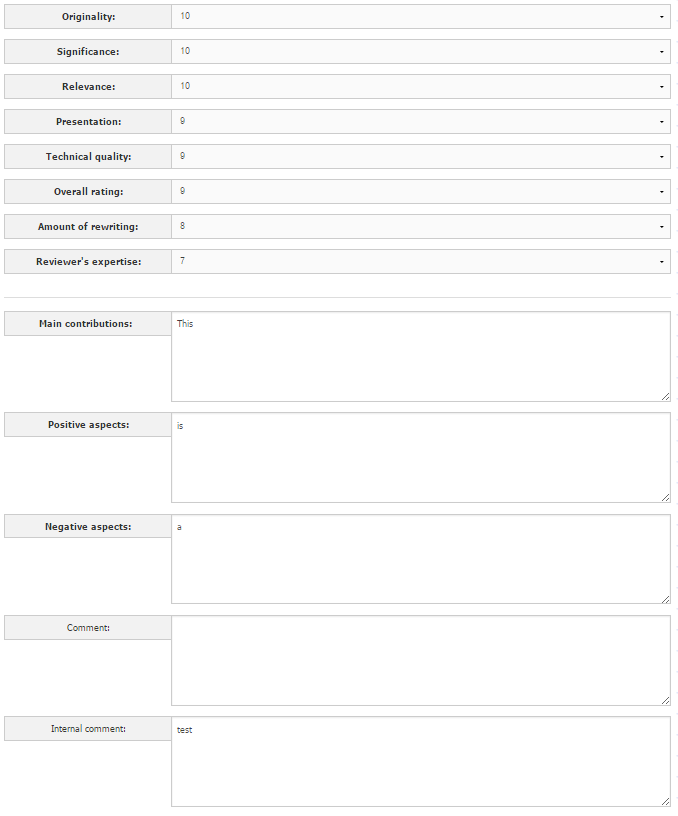
\includegraphics[width=0.5\textwidth]{obr8.png}
    	\caption{Vzhled webového formuláře}
    	\label{webform}
\end{figure}
V tomto formuláři je nejprve osm políček, ve kterých má uživatel možnost ohodnotit článek v rozmezí 0 až 10. Poté se ve formuláři nachází pět textových polí, kam uživatel vyplní své slovní hodnocení. 


\chapter{Dokumentace}
Konečná podoba mého modulu je realizována jako malá knihovna v jazyce PHP. Veškerý kód je rozdělen do dvou funkcí. Jedna se zabývá generováním PDF dokumentu a druhá jeho zpracováním. Také se v této knihovně na začátku nachází překrytá definice třídy z knihovny \emph{TCPDF}. 
\section{Třída PDFWithHeader}
Při vytváření PDF dokumentů pomocí knihovny \emph{TCPDF} se nejdříve volá konstruktor třídy \emph{TCPDF}. Danému objektu se poté nastavují parametry a vlastnosti pomocí jeho funkcí. Pokud však chceme změnit záhlaví nebo zápatí, je zapotřebí překrýt funkce \texttt{Header} a \texttt{Footer}. V našem případě není zapotřebí zápatí, proto překrývám jen funkci \texttt{Header}. Informace v záhlaví mohou být pokaždé jiné. 

Toto dynamické záhlaví je ve tvaru ID : Name. Proto potřebujeme naší překryté třídě nějakým způsobem předat tyto dvě informace. Rozhodl jsem se k tomu použít konstruktor, a tak jsem stávající konstruktor přetížil a přidal jsem 2 parametry - \texttt{Name} a \texttt{ID}. Tyto parametry se při volání konstruktoru uloží do vytvářeného objektu, podle návrhového vzoru \emph{přepravka} a jsou poté zpřístupněny z funkce \texttt{Header}.
\subsection{Funkce Header}
\label{lst:Header}
\begin{lstlisting}
public function Header() {
	$limit = 50;
	if(mb_strlen($this->name, 'UTF-8') > $limit){
		$this->name = mb_substr($this->name, 0, $limit, 'UTF-8')."... ";
	} 
	$this->SetFont('freesans', 'B', 20);
	$firstWordWidth = TCPDF::GetStringWidth($this->id ." : ", 'freesans', 'B', 20, false);
	$this->Cell($firstWordWidth, 0, $this->id ." : ", 0, 0, 'L', 0, '', 0, false, 'L', 'C');
	
	$this->SetFont('freesans', 'B', 15);
	$this->Cell(0, 0, $this->name , 0, 0, 'L', 0, '', 0, false, 'L', 'C');
	$this->Line(5, $this->y + 4, $this->w - 5, $this->y + 4);
}
\end{lstlisting}
V této funkci nejdříve dojde ke zkrácení proměnné \texttt{name}. Tato proměnná obsahuje název článku a často se stává, že je název článku příliš dlouhý. Text v záhlaví je vykreslován pomocí funkce \texttt{Cell}. Tato funkce text nezalamuje, to znamená, že pokud bychom nezkontrolovali jeho délku, došlo by po vykreslení k tomu, že by text pokračoval i mimo stránku. 

Veškeré objekty, které jsou vykreslovány pomocí knihovny \emph{TCPDF} se vykreslují na současnou pozici ukazatele. Tento pomyslný ukazatel se poté postupně posouvá. Pokud chceme jeho pozici nastavit, slouží k tomu funkce \texttt{setX} a \texttt{setY}. Pokud jsou tyto funkce použity se zápornými čísly, počítá se vzdálenost od pravé nebo spodní strany. Samotná funkce \texttt{Cell} má několik parametrů. 
\subsubsection{Funkce Cell a její parametry}
\begin{lstlisting}
$PDF->Cell(w, h, txt , border, ln, align, fill, link, stretch, ignore_min_height, calign, valign);
\end{lstlisting}
První dva parametry odpovídají šířce a výšce buňky, která bude vykreslena. Základní hodnoty těchto parametrů jsou 0. Buňka s~takovými parametry bude zabírat minimální výšku, do které se její obsah vejde, a maximální šířku. 

Dalším parametrem je samozřejmě text, který má buňka obsahovat. Poté následuje okraj. Tento parametr může nabývat číselných hodnot 0 a 1. Pokud je zvolena 1, je okraj buňky zvýrazněn černou čarou. Tato funkce je zvlášť užitečná při tvoření nových dokumentů, jelikož umožňuje zobrazení skutečného rozsahu dané buňky. Také je možné použít písmenné hodnoty L, T, R, B, které zobrazí okraj jen na jedné straně buňky. Písmena odpovídají anglickým názvům stran -- left, top, right a bottom. Například pokud bude parametrem řetězec "RTB", vykreslí se buňka, která bude mít okraj vpravo, nahoře a dole. Tato písmena mohou být v řetězci v jakémkoliv pořadí.

Parametr \texttt{ln} může nabývat hodnot 0 a 1. Tato možnost určuje, zda bude po vytisknutí buňky odřádkováno. Hodnota 1 je stejná jako volba 0 a okamžité použití funkce \texttt{Ln}. 

Další parametr \texttt{align} slouží k zarovnání textu. Tento parametr může nabývat hodnot L, C, R, J. Text bude tedy zarovnán vlevo, vycentrován a nebo zarovnán vpravo. Písmeno J znamená \emph{justify} a skrývá se pod ním takzvané \emph{zarovnání do bloku}. 

Parametr \texttt{fill} určuje, zda má být pozadí buňky průhledné nebo vyplněné. My budeme ve všech případech potřebovat, aby bylo průhledné, a tak bude nastaveno na \texttt{false}.

Pokud bychom potřebovali použít buňku jako hypertextový odkaz, použijeme k tomu parametr link. Lze do něj dosadit URL nebo identifikátor objektu vytvořeného funkcí \texttt{AddLink}.

Parametr \texttt{stretch} určuje chování textu v buňce a může nabývat pěti hodnot. Při hodnotě 0 je text zobrazen ve své velikosti a nedochází k žádnému zkreslení. Pokud je zadána hodnota 1, tak se text horizontálně zkrátí, pokud by se do dané buňky nevešel. Při hodnotě 2 se text přizpůsobí horizontálně velikosti buňky, i pokud by byl kratší. Pokud je zvolena hodnota 3, je dovoleno knihovně \emph{TCPDF} přizpůsobit i mezery mezi písmeny, tak aby se text do buňky vešel, a při hodnotě 4 jsou tyto mezery zvětšeny tak, aby text zabíral celý prostor buňky. 

Parametr \texttt{ignore\textunderscore min\textunderscore hight} lze použít, pokud chceme kreslit buňky menší než je jejich minimální výška, která je definovaná v knihovně \emph{TCPDF}. Tuto možnost také nebudeme potřebovat, takže ji necháme nastavenou na hodnotu \texttt{false}.

Parametry \texttt{calign} a \texttt{valign} oba určují vertikální zarovnání. První určuje vertikální zarovnání buňky a druhý textu, který buňka obsahuje. Parametr \texttt{calign} může nabývat hodnot T, C, B, A, L, D a parametr \texttt{valign} jen hodnot T, C, B. Všechny možné kombinace, kterých se dá docílit, jsou přehledně zobrazeny v obrázku \ref{zarovnani}. 

Pokud se tedy snažíme zarovnat celou buňku, můžeme použít například písmeno T. Toto písmeno reprezentuje slovo "Top" a buňka bude zarovnána tak, že její horní hranice bude umístěna na pomyslné linii, vytvořené horizontálně z bodu, od kterého obsah vykreslujeme. Ostatní písmena parametru \texttt{calign} reprezentují pozice "Center", "Bottom", "Ascent", "Baseline" a "Descent". Poslední tři pozice jsou určeny obsahem buňky. Jsou to linie nad textem, pod textem a linie, na které je text vykreslován. Toto je velice užitečné pokud se snažíme zarovnat buňky s~rozdílným nastavením písma a chceme, aby byl jejich obsah zarovnán na stejné úrovni. Parametr \texttt{valign} určuje pozici textu v buňce. Jednotlivá písmena reprezentují slova "Top", "Center" a "Bottom" a umožňují umístit text do buňky nahoru, doprostřed nebo dolů.
\begin{figure}[h]
    \centering
    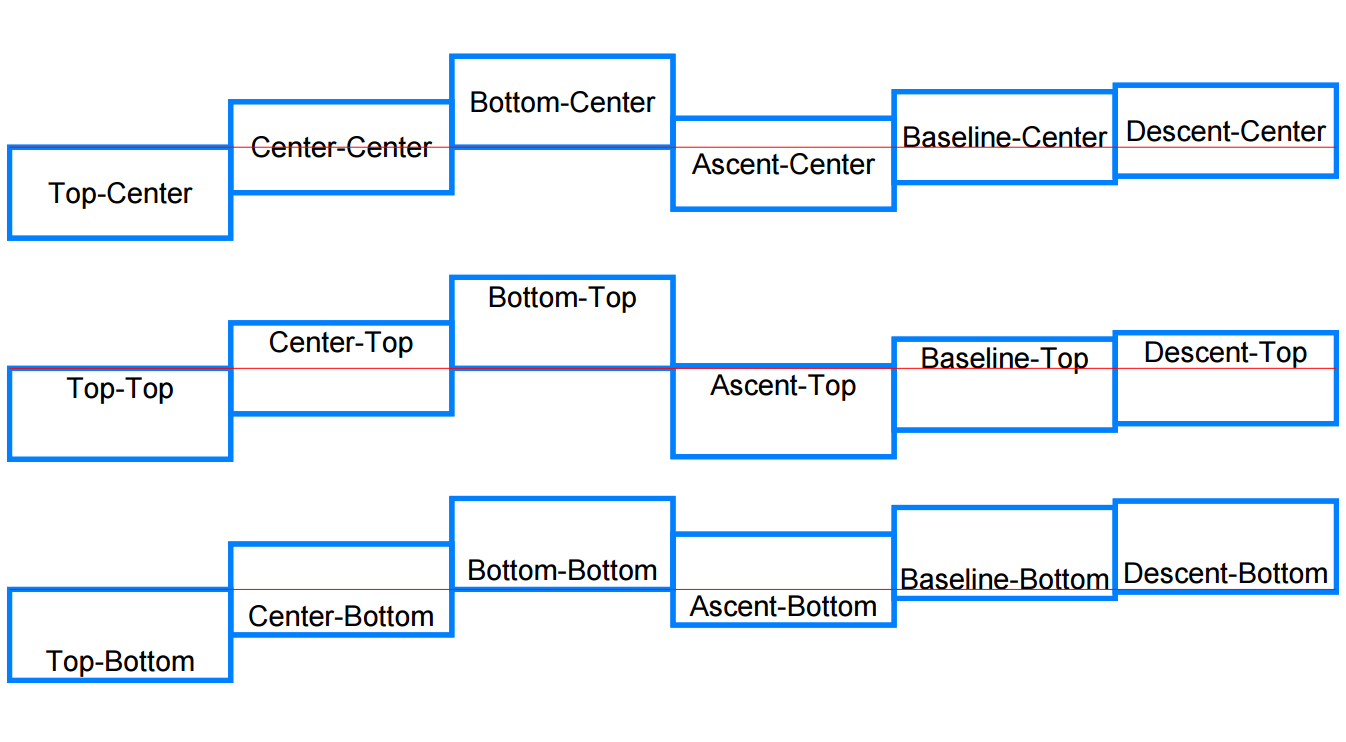
\includegraphics[width=0.75\textwidth]{obr1.png}
    \caption{Příklad vertikálního zarovnání buňky}
    \label{zarovnani}
\end{figure}

\section{Generování dokumentu}
\sloppy
Generování dokumentu probíhá ve funkci pojmenované \texttt{generate\textunderscore offline\textunderscore review\textunderscore form()}. Tato funkce má 6 parametrů. 
\label{lst:Generovani}
\begin{lstlisting}
function generate_offline_review_form($rid, $reviewer_name, $sid, $submission_name, $submission_filename, $review_html_footer)
\end{lstlisting}
\subsection{Parametry}
Parametr \texttt{rid} je identifikační číslo recenze. Portál TSD používá hned několik identifikačních čísel. Pro identifikaci uživatelů je používáno "User ID", pro identifikaci článků "Submission ID" a pro identifikaci recenzí "Review ID". \texttt{rid} je použito k propojení dat z PDF dokumentu a příslušným záznamem recenze v databázi. 

Jak již název napovídá, \texttt{reviewer\textunderscore name} je parametr obsahující celé jméno recenzenta, který daný článek hodnotí. Nejedná se tedy o autora článku, ale většinou o uživatele, který daný dokument stahuje. Každý článek, který je uložen na stránkách TSD, má přiřazeno své "Submission ID" a "User ID" autora. Tyto články jsou hodnoceny několika recenzenty. Vznikají tak recenze, které jsou identifikovány pomocí "Review ID" a "User ID" autora recenze. Může se stát, že recenzent nebude schopen svoji recenzi nahrát do systému TSD a odešle ji administrátorovi webových stránek. Ten bude schopen tuto recenzi do systému nahrát, i přestože není jeho. Parametr \texttt{reviewer\textunderscore name} se nachází v úvodním nadpisu i z důvodu, aby bylo okamžitě jasné, kdo danou recenzi vyplnil.

Parametr \texttt{sid} je identifikační číslo článku. Toto číslo musí být identické při generování a poté zpětném nahrávání. Pokud by tato čísla nebyla stejná, odhalila by to kontrola při nahrávání souboru a znamenalo by to problém v konzistenci dat. K této chybě by mohlo dojít, pokud by se například změnil obsah databáze poté, co byl soubor stažen a předtím, než byl do systému opět nahrán. Znamená to také, že článek, ke kterému byla recenze vygenerovaná, byl mezitím odstraněn z databáze. Toto je chyba, kterou běžný uživatel neuvidí, protože současná webová stránka TSD ani neumožňuje nahrát recenzi neexistujícímu článku.  

Parametr \texttt{submission\textunderscore name} je celý název článku, který daná recenze hodnotí. Pokud je tento název dlouhý, tak že by se nevešel do vyhrazeného místa, dojde ke zkrácení a zbytek textu bude nahrazen třemi tečkami. 

Parametr \texttt{submission\textunderscore filename} je celá cesta k originálnímu dokumentu článku ve formátu PDF. Pokud by se v dané cestě nenacházel soubor ve formátu PDF, dojde pouze k vygenerování formuláře.

Poslední parametr \texttt{review\textunderscore html\textunderscore footer} slouží k definici vlastního zápatí poslední stránky. Obsahem této proměnné musí být řetězec obsahující HTML kód. 
\subsection{Generování}
Funkce pro generování dokumentu využívá hned několik nástrojů. K vytváření nových dokumentů je použita knihovna \emph{TCPDF}. S~již existujícími dokumenty je manipulováno pomocí nástroje \emph{PDFToolkit} a formulář je navržen pomocí nástroje \emph{Adobe FormsCentral}. 

Ve funkci pro generování, která je zobrazena v kapitole \ref{lst:Generovani} jsou nejprve definovány názvy všech dočasných souborů, které budou následně využity. Poté dojde ke kontrole typu souboru článku. Pokud se jedná o PDF, tak dojde ke sloučení již existujícího souboru s~formulářem a daného PDF souboru s~článkem. Naopak pokud se o PDF soubor nejedná, tak bude kód funkce pokračovat pouze se samotným formulářem.
\subsubsection{Sloučení}
Při slučování dochází ke spojení dvou PDF dokumentů. Například pokud mám titulní stranu mé práce v dokumentu na obrázku \ref{titulni_strana} a chtěl bych ji sloučit s~existujícím článkem, který je v dokumentu na obrázku \ref{clanek}.
\begin{figure}[h]
    \centering
    \begin{minipage}[b]{0.4\textwidth}
    	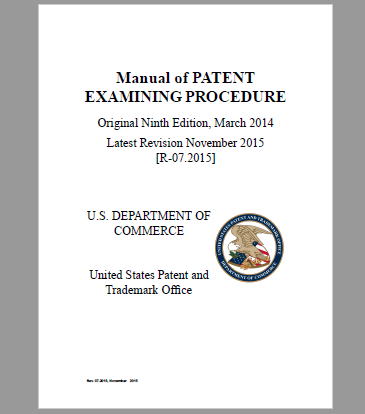
\includegraphics[width=\textwidth]{obr2.png}
    	\caption{Dokument s~titulní stranou}
    	\label{titulni_strana}
    \end{minipage}
    \hfill
    \begin{minipage}[b]{0.4\textwidth}
    	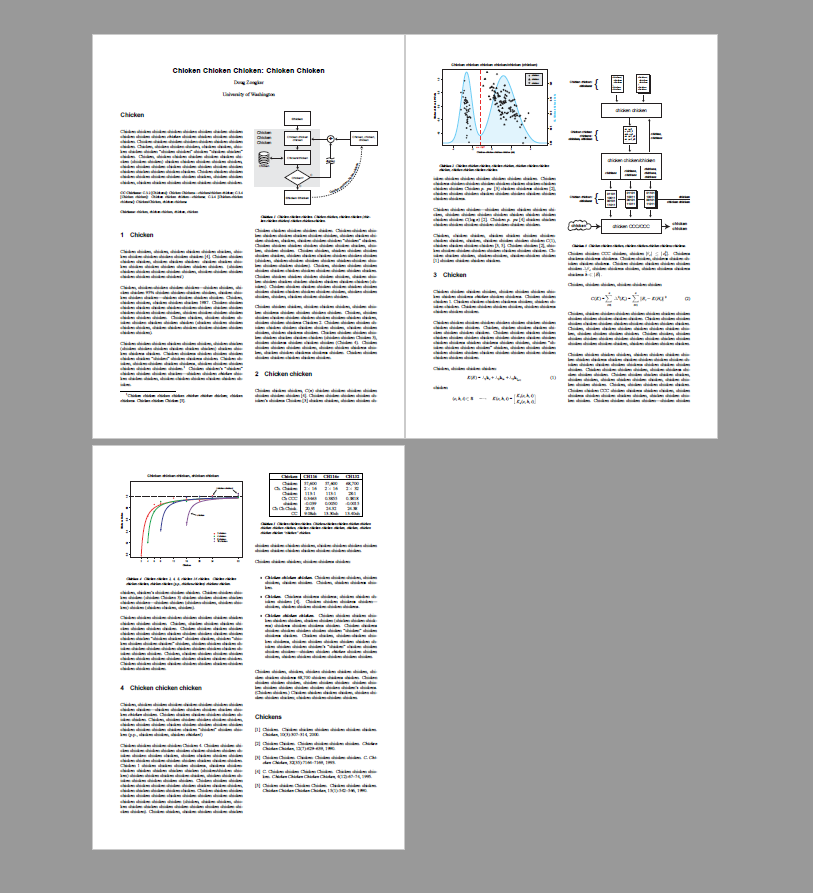
\includegraphics[width=\textwidth]{obr3.png}
    	\caption{Dokument s~článkem}
    	\label{clanek}
    \end{minipage}
\end{figure}
Mohu k tomu použít příkaz nástroje \emph{PDFToolkit}.
\begin{lstlisting}
pdftk title.pdf submission.pdf cat output combined.pdf
\end{lstlisting}
Pokud dokument \texttt{title.pdf} je dokument z obrázku \ref{titulni_strana} a \texttt{submission.pdf} je dokument z obrázku \ref{clanek} pak výsledným dokumentem bude obrázek \ref{kombinace}
\begin{figure}[h]
    \centering
    	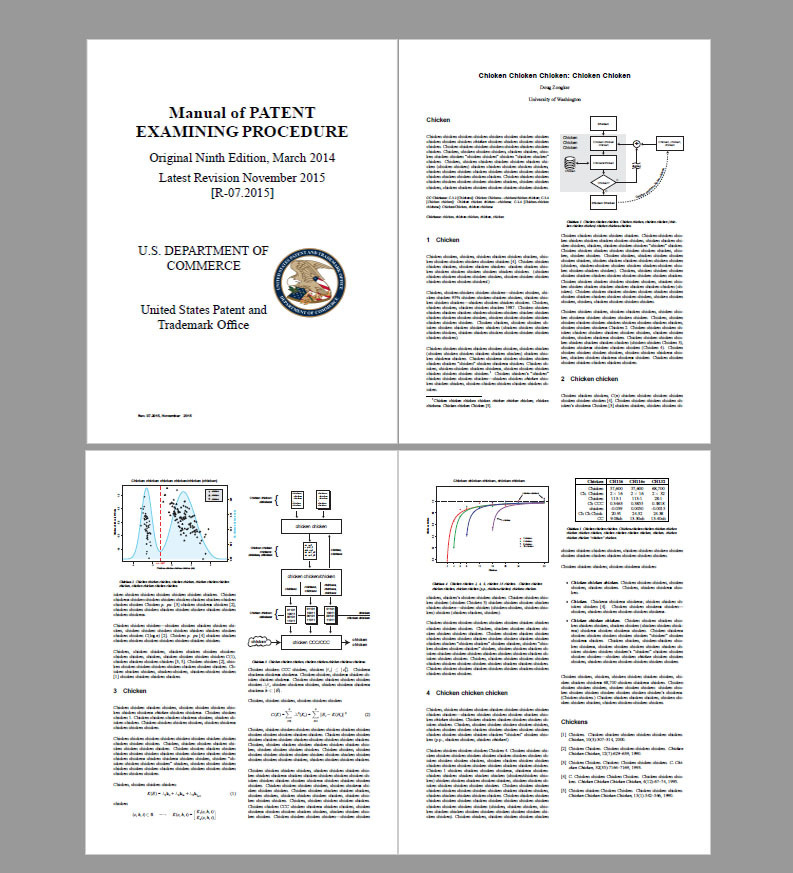
\includegraphics[width=0.5\textwidth]{obr5.jpg}
    	\caption{Výsledný dokument}
    	\label{kombinace}
\end{figure}
\subsubsection{Prokládání}
Dále je zapotřebí přidat záhlaví s~informacemi o recenzi. K tomu je využita již výše zmíněná třída PDFWithHeader. Vytvoříme tedy jednu stránku s~žádaným záhlavím a poté tento dokument vykreslíme. Máme tedy formulář s~článkem v jednom dokumentu a záhlaví v druhém. Ke spojení použijeme nástroj PDFToolkit, který umožňuje prokládání již existujících dokumentů. Proložení je docíleno tímto příkazem. 
\begin{lstlisting}
pdftk withoutHeader.pdf multistamp header.pdf output combined.pdf
\end{lstlisting}
Pokud bychom se snažili prokládat dva soubory, přičemž \texttt{withoutHeader.pdf} je dokument na obrázku \ref{withoutHeader} a \texttt{header.pdf} se podobá dokumentu na obrázku \ref{header}, vznikl by dokument s~názvem \texttt{combined.pdf}, který bude vypadat jako dokument na obrázku \ref{kombinace2}.

\begin{figure}[h]
    \centering
    \begin{minipage}[b]{0.4\textwidth}
    	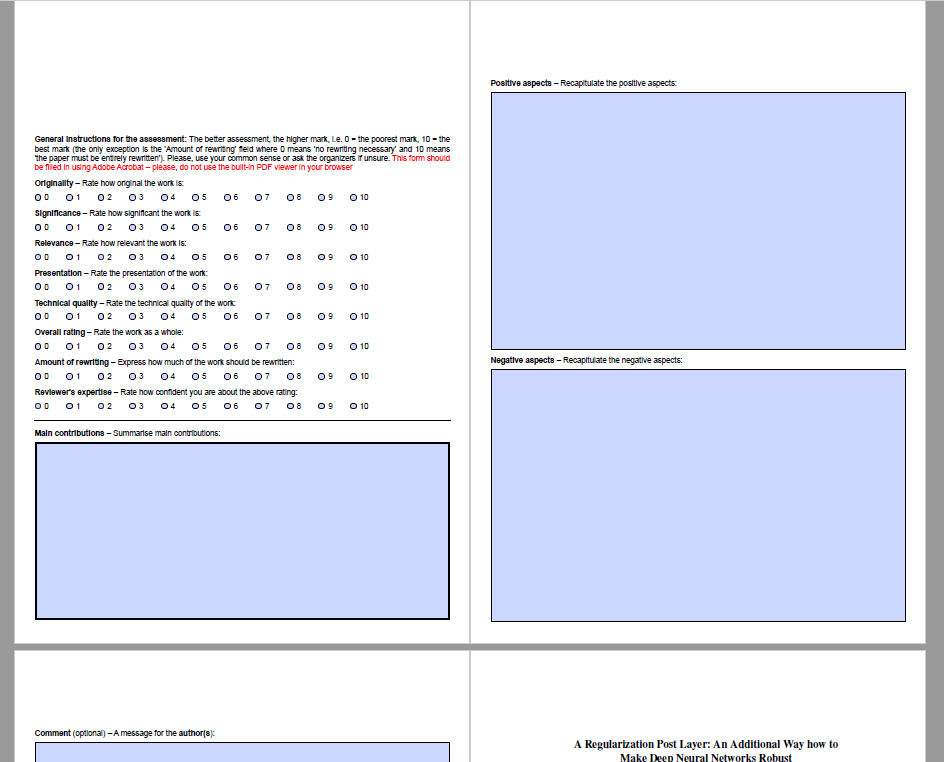
\includegraphics[width=\textwidth]{obr5.png}
    	\caption{Dokument bez záhlaví}
    	\label{withoutHeader}
    \end{minipage}
    \hfill
    \begin{minipage}[b]{0.4\textwidth}
    	
\includegraphics[width=\textwidth]{obr6.png}
    	\caption{Záhlaví dokumentu}
    	\label{header}
    \end{minipage}
\end{figure}
\begin{figure}[h]
    \centering
    	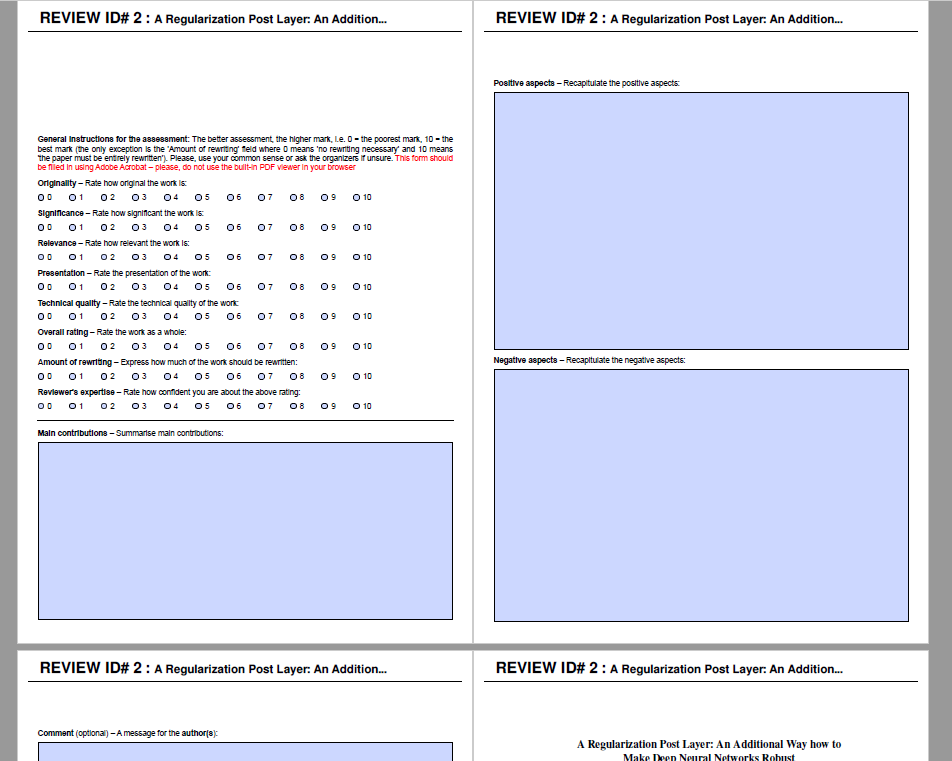
\includegraphics[width=0.8\textwidth]{obr7.png}
    	\caption{Výsledný dokument bez nadpisu}
    	\label{kombinace2}
\end{figure}
\subsubsection{Nadpis}
Následně se pomocí knihovny \emph{TCPDF} vytvoří další PDF soubor obsahující pouze hlavní nadpis. Tento soubor bude stejným způsobem proložen již existujícím PDF souborem, obsahujícím formulář, článek a teď i záhlaví. Jelikož chceme, aby nástroj \emph{PDFToolkit} takto spojil jen první stránku, na které se nadpis nachází, je nutné, aby byl dokument s~nadpisem ukončen prázdnou stránkou. \emph{PDFToolkit} totiž při prokládání postupuje po stránkách, a pokud má dokument stránek méně, dojde k opakování poslední strany. Pokud má tedy soubor s~nadpisem jen jedinou stránku, bude tento nadpis proložen všemi stranami výsledného dokumentu, stejně jako tomu bylo u záhlaví. 

V této chvíli jsme získali dokument s~formulářem, připojeným článkem, záhlavím a nadpisem. Od finálního vzhledu nás dělí jen zápatí na poslední stránce. Opět tedy vytvoříme dokument pomocí knihovny \emph{TCPDF}. Tentokrát bude obsahovat dvě prázdné stránky, třetí stránku obsahující zápatí a ukončovací prázdnou stránku. Proložením získáme již kompletní dokument se všemi informacemi. Tomuto dokumentu je ještě zapotřebí upravit metadata. Nejdříve tedy použijeme \emph{PDFToolkit} na extrakci současných dat do souboru. K těmto datům poté přidáme identifikační čísla článku a recenze a tímto příkazem aktualizujeme metadata: 
\begin{lstlisting}
PDFtk withoutMeta.PDF update_info metafile.txt output withMeta.PDF
\end{lstlisting}
Výsledný soubor je již finální, a tak ho odešleme prohlížeči ke stažení.
\section{Zpracování dokumentu}
Zpracování dokumentu je realizováno touto funkcí s~3 parametry.
\begin{lstlisting}
function process_offline_review_form($rid, $sid, $revform_filename) 
\end{lstlisting}
\subsection{Parametry}
Prví dva parametry, \texttt{rid} a \texttt{sid}, obsahují identifikační čísla článku a recenze. Jsou zde pouze pro kontrolu, zda uživatel nahrává správný soubor do správné recenze na webu TSD. Třetím parametrem je cesta k PDF dokumentu, který byl nahrán na server.
\subsection{Zpracování}
Při zpracování dojde nejprve k extrakci identifikačních čísel článku a recenze ze souboru. Tyto hodnoty jsou následně porovnány s~čísly, které byly zadány jako parametry funkce pro zpracování. Pokud se liší číslo recenze, pravděpodobně se uživatel snaží pouze nahrát dokument s~recenzí k jinému článku, než zvolil ve webové aplikaci. Pokud se však liší číslo článku, jedná se o chybu konzistence. Nikdy by se totiž nemělo změnit identifikační číslo článku, bez změny čísla recenze. Po této kontrole jsou extrahována pomocí nástroje PDFToolkit datová pole. Výstup s~informacemi o datových polích může vypadat například takto:
\label{vystup}
\begin{lstlisting}[basicstyle=\footnotesize,caption={Ukázka výstupu nástroje PDFToolkit},label={lst:vystup}]
---
FieldType: Button
FieldName: Originality &#8211; Rate how origina_ir*LeqwssF5KR7JiEO01FA
FieldFlags: 49152
FieldValue: 1
FieldJustification: Left
FieldStateOption: 0
FieldStateOption: 1
FieldStateOption: 10
FieldStateOption: 2
FieldStateOption: 3
FieldStateOption: 4
FieldStateOption: 5
FieldStateOption: 6
FieldStateOption: 7
FieldStateOption: 8
FieldStateOption: 9
FieldStateOption: Off
---
FieldType: Text
FieldName: Internal comment (optional) &#8211; _rKkqBCjQ4mH7ygxrjhFaFw
FieldNameAlt: Internal comment (optional) &#8211; An internal message for the organizers:
FieldFlags: 4096
FieldValue: Text kter&#253; je obsa&#382;en v textov&#233;m poli Intern&#237; koment&#225;&#345;.
FieldJustification: Left
---
FieldType: Text
FieldName: fc-int01-generateAppearances
FieldFlags: 5
FieldJustification: Left
\end{lstlisting}
Jednotlivá datová pole jsou oddělena skupinou tří pomlček. Informace o datových polí jsou rozděleny pod \emph{tokeny}, jako \texttt{FieldType}, \texttt{FieldName} a \texttt{FieldValue}. Dojde tedy k parsování a výsledné pole hodnot je předáno další funkci, která komunikuje s~databází. 
\subsection{Parsování}
Po získání výstupu z programu \emph{PDFToolkit} dojde k parsování. Soubor je načten do proměnné \texttt{\$text}. Tento výstup, který je zobrazen v ukázce \ref{lst:vystup}, je zpracován cyklem \ref{lst:parser}. Tento cyklus postupně prochází proměnnou \texttt{\$text} a snaží se získat počáteční a koncové pozice textu, který se nachází za \emph{tokeny} \texttt{FieldName:} a \texttt{FieldValue:}. Tyto \emph{tokeny} jsou parametry jednotlivých datových polí PDF dokumentu. Datová pole jsou ve výpisu oddělena pomocí řetězce \texttt{-}\texttt{-}\texttt{-}. Může se stát, že bude dokument PDF obsahovat i datová pole, která tyto \emph{tokeny} neobsahují. Pokud k tomu dojde, \emph{parser} dané datové pole přeskočí a pokračuje dalším polem.  
\begin{lstlisting}[basicstyle=\scriptsize,caption={Parsovací cyklus},label={lst:parser}]
//pole do ktereho budou ulozeny nalezene hodnoty
$arr = array();	
//urcuje pozici, od ktere je hledano datove pole, zvetsuje se podle poctu jiz zpracovanych datovych poli v textu
$fieldPos = 0;	
//cyklus probiha dokud vystup obsahuje token "---"
while (($fieldPos = strpos($text, "---".PHP_EOL, $fieldPos))!== false) {	
    $fieldPos  = $fieldPos  + strlen("---".PHP_EOL);
    $fieldSize = strpos($text, "---".PHP_EOL, $fieldPos) - strlen("---".PHP_EOL);
    //pozice zacatku datoveho pole
    $field = substr($text, $fieldPos, $fieldSize - $fieldPos);	
    $fieldName = strpos($field, "FieldName: ", 0);
    //pokud neobsahuje datove pole token "FieldName:" cyklus pokracuje dalsim polem
    if($fieldName === false){	
        continue;
    }
    $fieldName += strlen("FieldName: ");
    $fieldNameSize = strpos($field, PHP_EOL, $fieldName) - $fieldName;
    //ziskani nazvu datoveho pole
	$key = substr($field, $fieldName, $fieldNameSize);	
	//kdyz neni datove pole vyplneno je nastaveno na NULL 
	$arr[$key] = NULL;	
    $fieldValue = strpos($field, "FieldValue: ", $fieldName);
    //pokud neobsahuje datove pole token "FieldValue:" cyklus pokracuje dalsim polem
    if($fieldValue === false){	
        continue;
    }
    $fieldValue += strlen("FieldValue: ");
    $fieldValueSize = strpos($field, PHP_EOL, $fieldValue) - $fieldValue;
    //ziskani hodnoty datoveho pole
	$value = substr($field, $fieldValue, $fieldValueSize);	
	//kdyz je datove pole vyplneno dojde k ulozeni hodnoty do pole 
	   $arr[$key] = $value;	
}
\end{lstlisting}
\subsection{Aktualizace hodnot v databázi}
\sloppy
Poslední funkce, která je při zpracování dokumentu použita se nazývá \texttt{upload\textunderscore to\textunderscore DB\textunderscore offline\textunderscore review\textunderscore form()}. Tato funkce nejdříve zkontroluje, zda jsou předané hodnoty korektní. Uživatel se může pokusit nahrát dokument s~recenzí, která byla již označena jako uzavřená, proto je nejdřív získán současný stav recenze, kterou se snažíme aktualizovat. Pokud je stav vyhovující, dojde k uložení všech hodnot do databáze. 
\chapter{Rozšiřitelnost}
Ve složce se zdrojovým kódem je umístěn vyplnitelný formulář, který je používán při generování dokumentů. Pokud je tento dokument nahrazen jiným formulářem vytvořeným pomoci programu \emph{Adobe FormsCentral}, budou výsledné dokumenty obsahovat tento upravený formulář. Z toho důvodu složka obsahuje i soubor s~koncovkou \emph{.fcdt}.

Jedná se totiž o šablonu, pomocí které byl první formulář vytvořen. Stačí tedy tento soubor otevřít pomocí \emph{Adobe FormsCentral}, provést změny a vygenerovat nový formulářový dokument ve formátu PDF. 
\sloppy

Při větších úpravách se však nevyhneme zásahům do kódu. Pokud se například změní počet polí, je nutné aktualizovat příkaz, který ukládá hodnoty do databáze. Veškerá práce s~databází se nachází ve funkci \texttt{upload\textunderscore to\textunderscore DB\textunderscore offline\textunderscore review\textunderscore form()}. Také je nutné si uvědomit, že informační zápatí formuláře bude vždy vykresleno na třetí straně dokumentu. Pokud se tedy počet stránek formuláře změní, je nutné ubrat, popřípadě přidat prázdné stránky z generovaného dokumentu obsahujícího zápatí.

Druhý přístup, na který jsem bohužel přišel příliš pozdě, je generování celého formuláře pomocí knihovny \emph{TCPDF}. Když jsem při prvotním průzkumu tuto možnost zkoušel, nedokázal jsem najít způsob, jak získat data z formulářů vytvořených pomocí knihovny \emph{TCPDF}. To se mi podařilo až s~formulářem vytvořeným pomocí \emph{Adobe FormsCentral}. Navíc jsem si v té době naplno neuvědomoval, jak bude můj modul reálně nasazen. Až při testování jsem přišel na to, že \emph{PDFToolkit} dokáže zjistit obsah i datových polí vytvořených knihovnou \emph{TCPDF}. Jsem přesvědčen o tom, že tento přístup je korektnější, proto se v této části pokusím vysvětlit postup, jak navrhnout vyplnitelné formuláře pomocí knihovny \emph{TCPDF}.
\section{Formuláře v TCPDF}
Tvorba formulářů knihovnou \emph{TCPDF} je opravdu jednoduchá. Velmi se podobá tvorbě klasických statických dokumentů. Nejprve je nutné vytvořit objekt \texttt{TCPDF}, do kterého můžeme následně začít vykreslovat buňky s~textem.
\begin{lstlisting}
$PDF = new TCPDF();
$PDF->AddPage();
$PDF->SetFont('helvetica', 'BI', 18);
$PDF->Cell(0, 5, 'Priklad formulare', 0, 1, 'C');
$PDF->Ln(10);
\end{lstlisting}
Funkce \texttt{Cell} vykreslí na současnou pozici text "Priklad formulare" a poté dojde k odřádkování pomocí funkce \texttt{Ln}. Pomocí knihovny \emph{TCPDF} je dále možné vytvořit textová pole, přepínače, zatrhávací políčka nebo například tlačítka. Všem těmto prvkům je přiřazeno jméno, díky kterému je možné s~obsahem manipulovat pomocí \emph{JavaScriptu}. To lze například využít k validaci ze strany uživatele. 
\subsection{Příklad validace formuláře pomocí JavaScriptu}
Pokud bychom chtěli kontrolovat formulář pomocí \emph{JavaScriptu}, je možné k tomu použít kód podobající se tomuto příkladu. 
\begin{lstlisting}
$pdf->Button('tisk', 30, 10, 'Tisk', 'Tisk()', array('lineWidth'=>2, 'borderStyle'=>'beveled', 'fillColor'=>array(128, 196, 255), 'strokeColor'=>array(64, 64, 64)));
$js = <<<EOD
function Zkontroluj(pole,zpravaProUzivatele) {
    var f = getField(pole);
    if(f.value == '') {
        app.alert(zpravaProUzivatele);
        f.setFocus();
        return false;
    }
    return true;
}
function Tisk() {
    if(!Zkontroluj('jmeno','Vyplnte jmeno')) {return;}
    if(!Zkontroluj('prijmeni','Vyplnte prijmeni')) {return;}
    if(!Zkontroluj('pohlavi','Vyplnte pohlavi')) {return;}
    if(!Zkontroluj('adresa','Vyplnte adresu')) {return;}
    print();
}
EOD;
$pdf->IncludeJS($js);
\end{lstlisting}
Nejdříve vytvoříme tlačítko, které bude v tomto případě tisknout náš PDF dokument. Toto tlačítko při stisknutí volá funkci \texttt{Tisk()}. Kód \emph{JavaScript}, který budeme chtít v dokumentu použít, musí být předán jako řetězec funkci \texttt{IncludeJS()}. Funkce \texttt{Tisk()} tedy postupně volá funkci \texttt{Zkontroluj()} nad textovými poli, které mají identifikátory \texttt{jmeno}, \texttt{prijmeni}, \texttt{pohlavi} a \texttt{adresa}. Funkce \texttt{Zkontroluj()} pouze porovná obsah textového pole s~prázdným řetězcem. Pokud uživatel do pole nic nevyplnil zobrazí se mu upozornění se zprávou. Pokud jsou všechna pole vyplněna dojde k vytisknutí dokumentu pomocí funkce \texttt{print()}.
\subsection{Tvorba formuláře}
Pokud bychom chtěli přizpůsobit vzhled formuláře, můžeme k tomu použít funkci \texttt{setFormDefaultProp}, která nám umožní definovat vlastní okraje nebo například barvu textových polí. 
\begin{lstlisting}[firstnumber=6]
$PDF->setFormDefaultProp(array('lineWidth'=>1, 'borderStyle'=>'solid', 'fillColor'=>array(255, 255, 200), 'strokeColor'=>array(255, 128, 128)));
\end{lstlisting}
Dále do dokumentu přidáme formulářové prvky. Pro vytvoření textového pole použijeme funkci \texttt{TextField}. Nejdříve přidáme popis textového pole, za něj vykreslíme samotné textové pole a poté opět odřádkujeme.
\begin{lstlisting}[firstnumber=7]
$PDF->Cell(35, 5, 'Textove pole:');
$PDF->TextField('field01', 50, 5);
$PDF->Ln(6);
\end{lstlisting}
První parametr funkce \texttt{TextField} je identifikátor. Ten je následován šířkou a výškou textového pole. Poté do dokumentu přidáme seznam, pomocí funkce \texttt{ComboBox}.
\begin{lstlisting}[firstnumber=10]
$PDF->Cell(35, 5, 'Vyberove pole:');
$PDF->ComboBox('field02', 30, 5, array(array('', '-'), array('M', 'Muz'), array('Z', 'Zena')));
$PDF->Ln(6);
\end{lstlisting}
První parametry jsou totožné, čtvrtý parametr je pole polí, které obsahuje všechny možnosti, které může uživatel při vyplňování zvolit. Dále přidáme několik přepínačů.
\begin{lstlisting}[firstnumber=13]
$PDF->Cell(35, 5, 'Prepinace:');
$PDF->RadioButton('field03', 5, array(), array(), 'Zvolil 1');
$PDF->Cell(35, 5, 'Jedna');
$PDF->Ln(6);
$PDF->Cell(35, 5, '');
$PDF->RadioButton('field03', 5, array(), array(), 'Zvolil 2', true);
$PDF->Cell(35, 5, 'Dva');
$PDF->Ln(6);
$PDF->Cell(35, 5, '');
$PDF->RadioButton('field03', 5, array(), array(), 'Zvolil 3');
$PDF->Cell(35, 5, 'Tri');
$PDF->Ln(6);
\end{lstlisting}
Pokud chceme, aby měl uživatel na výběr z několika možností, je důležité, aby měly přepínače stejný identifikátor. Druhý parametr funkce \texttt{RadioButton} je velikost přepínače, ta je následována poli, ve kterých je možné upřesnit vlastnosti a parametry, které lze využít při práci s~\emph{JavaScriptem}. 

Jelikož my v našem formuláři \emph{JavaScript} nepoužijeme, můžeme toto pole nechat prázdná. Pátý parametr je hodnota, která bude uložena při zvolení dané možnosti. Jako šestý parametr je možné zadat výchozí hodnotu. V našem případě bude po otevření souboru předem zvolena druhá možnost. Další prvek, který můžeme do našeho formuláře přidat, je zaškrtávací políčko:
\begin{lstlisting}[firstnumber=25]
$PDF->Cell(35, 5, 'Zaskrtavaci policko:');
$PDF->CheckBox('field04', 5, true, array(), array(), 'Zaskrtnuto');
$PDF->Ln(6);
\end{lstlisting}
Zaškrtávací políčko se podobá přepínači, pouze je změněno pořadí a výchozí stav pole je definován jako třetí parametr místo šestého. Poté, co vytvoříme pomocí předchozích funkcí náš formulář, je ještě nutné definovaný obsah vykreslit. K tomu použijeme funkci \texttt{Output}.
\begin{lstlisting}[firstnumber=28]
$PDF->Output('formular.PDF', 'D');
\end{lstlisting}
Druhý parametr této funkce určuje, kam má být výsledný dokument odeslán. Pokud je zvoleno \texttt{D}, bude soubor odeslán webovému prohlížeči. Druhá možnost je například zvolit \texttt{F}, poté bude soubor uložen lokálně na serveru.
Dokument, který je vytvořen tímto skriptem, je poté možno opět umístit do složky s~modulem, který ho začne využívat ke generování dokumentů s~recenzí. Poté je opět nutno zkontrolovat obsah pole, které vznikne po parsování výstupu nástroje \emph{PDFToolkit} a přizpůsobit mu funkci pro ukládání hodnot do databáze.
\chapter{Testování}
Vytvořený modul bylo nutné také otestovat. 
\section{Kompatibilita}
\subsection{Webové prohlížeče}
Nejprve jsem se rozhodl otestovat kompatibilitu s~různými internetovými prohlížeči. 

Prvním prohlížečem, který jsem testoval, byla \emph{Mozilla Firefox} verze 47.0.1. V tomto prohlížeči proběhlo vše správně. Po stažení souboru se objevilo dialogové okno prohlížeče, které umožnilo uživateli otevřít soubor PDF v doporučeném programu \emph{Acrobat Reader}. A zpětné nahrání opět proběhlo bez problému. 

Dalším prohlížečem byl \emph{Microsoft Edge 40}, který je v dnešní době nainstalován jako výchozí prohlížeč na počítačích používajících operační systém \emph{Microsoft Windows 10}. I prohlížeč \emph{Edge} neměl se stažením a zobrazením nejmenší problém. 

Poté jsem stažení otestoval i na prohlížeči \emph{Internet Explorer 11}. Ten, podobně jako \emph{Edge}, zobrazil dialogové okno, které umožnilo otevření dokumentu v programu \emph{Acrobat Reader}. 

Jako poslední jsem otestoval nejpoužívanější prohlížeč \emph{Google Chrome} verze 57.0. U něj jsem narazil na problém. \emph{Google Chrome} totiž umožňuje zobrazení obsahu PDF dokumentů ve vestavěném prohlížeči. Poté co jsem se pokusil otevřít stažený dokument, otevřela se nová záložka, ve které se dokument s~formulářem zobrazil. Tento vestavěný prohlížeč dokonce umožňuje i vyplnění obsahu formuláře. Vyplněná data by se měla ukládat do souboru. Jelikož však \emph{Google Chrome} otevírá jen náhled, není možné otevřený soubor měnit. Pokud by uživatel chtěl vyplnit recenzi online, je k tomu na stránkách TSD určen webový formulář, proto nedává smysl vyplňování offline PDF furmuláře pomocí webového prohlížeče. Aby nedocházelo k nedorozumění, byl do záhlaví PDF formuláře raději přidán informační text, který upozorňuje uživatele, aby formulář raději vyplnil pomocí programu \emph{Acrobat Reader}.
\subsection{Editory}
Vyplnění formuláře bylo otestováno jak v bezplatné verzi programu \emph{Acrobat Reader DC 17.9}, tak v placené verzi \emph{Adobe Acrobat 11}. Obě verze umožnily bezproblémové vyplnění a uložení formuláře. Otestoval jsem i speciální znakové sady. 

Pokud chce uživatel vyplnit formulář například v angličtině nebo češtině, nedochází k žádnému problému. Uživatel může dokonce do formuláře vložit i speciální znaky, které se nacházejí v UTF-8. Při psaní těchto znaků si program Acrobat Reader sám dohledá a nainstaluje potřebné rozšíření. 

To, co je možné do formuláře vyplnit, není tedy omezeno formátem souboru, ale spíše verzí a rozšířením programu Acrobat Reader, kterým uživatel dokument vyplňuje. Co se týče velikosti, je tento formát skoro bez omezení. Uživatel může do textových polí vložit klidně několik stránek textu a nedojde k žádnému drastickému snížení rychlosti. 

Dále bylo vyplnění formuláře otestováno i na operačním systému Linux v prohlížeči dokumentů \emph{Evince} verze 2.32.0.145. Tento prohlížeč dosáhl podobných výsledků jako programy od firmy Adobe. Vyplnění a uložení formuláře proběhlo bez problému.
\section{Generování a nahrávání}
Při testování generování a nahrání mě zajímala především rychlost. Autoři článků, mohou do databáze uložit soubory o libovolné velikosti. Obával jsem se, že pokud budou tyto články, které se připojují k formuláři, příliš velké, dojde ke zpomalení. To se však nestalo. Zpracování bylo otestováno s~PDF souborem o velikosti 10 MB. Ke zpomalení došlo spíše kvůli rychlosti internetového připojení, než samotnou prací mého modulu. 
\section{Odhalené chyby}
Během testování bylo odhaleno několik chyb. Ty nejzajímavější jsem se rozhodl popsat v této sekci.
\subsection{Diakritika v nadpisu}
Při vytváření textů jsem se soustředil na to, aby bylo možné vygenerovat dokumenty s~českou diakritikou. Formuláře, které jsem generoval, měly v nadpisu mé jméno, které obsahovalo písmeno \uv{á}. Až pozdější testy ukázaly, že skript nedokázal vykreslit všechny diakritické znaky české abecedy. Naštěstí to nebyl problém v kódování, ale v použitém fontu. Základní fonty, které knihovna \emph{TCPDF} používá, českou diakritiku neumí.

Žádný z nich však neobsahuje znaky pro českou diakritiku. Naštěstí je součástí knihovny \emph{TCPDF} více fontů, o kterých v dokumentaci není zmínka. Fonty \emph{freesans} a \emph{freeserif} dokáží zobrazit i českou diakritiku, a tak jsou ideální pro náš modul. Pokud je nutné generovat české texty, doporučuji jejich využití. \emph{freesans} je bezpatkové písmo a \emph{freeserif} je patkové.
\subsection{Speciální znaky ve formuláři}
Program \emph{Acrobat Reader} umožňuje uživateli vyplnit do formuláře jakékoliv znaky. Při testování jsem zjistil, že tyto znaky nemusí být kompatibilní s~nastavením tabulky v databázi, a proto jsem přidal kontrolu. Při neúspěchu se uživateli zobrazí chybová hláška. Tato chyba však nastane jen ve velmi extrémních případech, když se uživatel snaží vyplnit do formuláře například emotikony a jiné neobvyklé znaky. 
\subsection{Nekorektně vyplněný formulář}
V první verzi mého modulu mohl uživatel vyplnit svůj formulář jakkoliv. Při nahrávání poté došlo k přepisu původní verze recenze tou novou. To, že mohl uživatel nahrát i formulář jen s~jedním vyplněným polem, by mohlo být potenciálně matoucí. Uživatel by mohl předpokládat, že nahráním dalšího formuláře, který obsahuje ostatní pole, dojde ke sloučení. Ve skutečnosti však dojde k přepsání původní odpovědi odpovědí novou. Z toho důvodu jsem raději přidal kontrolu, která zjišťuje, zda byl formulář vyplněn kompletně a žádná povinná pole nebyla vynechána. Současně jsem také přidal kontrolu rozsahu hodnot odpovědí. Uvědomil jsem si totiž, že pokud má uživatel na výběr z rozsahu hodnot 1-10, je možné upravit formát souboru a nahrát tak číslo mimo tento rozsah, i pokud mu to neumožňuje vzhled formuláře. 
\subsection{Nahrání jiného PDF}
Další chyba, která byla odhalena až testováním, bylo zvolení PDF, které nebylo vygenerováno jako recenze pro článek TSD. Když jsem vytvářel první verzi, tak jsem si neuvědomil, že by se uživatel mohl pokusit nahrát soubor, který neobsahuje námi vygenerovaný formulář PDF. Samozřejmě by tím ničeho nedocílil, protože by soubor nešel zpracovat. Modul by však selhal s~jinou chybovou hláškou, a tak by mohl uživatele zmást. Přidal jsem tedy další chybovou hlášku, která uživatele informuje o nahrání nekorektního souboru. 
\subsection{Špatný posun při parsování}
Chyba, která se hledala nejhůře, byla chyba v parsování textu. Byla to současně chyba, na kterou jsem přišel až poměrně pozdě. Parsování textu totiž na první pohled vypadalo funkčně a bezchybně. Velké množství testů prošlo bez problémů, pouze jediný měl zvláštní výsledek. V tomto testu byla vyplněna všechna pole až na pole předposlední. Při nahrání tohoto formuláře do databáze došlo k duplikaci poslední hodnoty i na místo předposlední. Díky tomuto testu jsem si uvědomil, že můj cyklus může v tomto speciálním případě načíst hodnotu nesprávného pole. Modul jsem opět upravil tak, aby ukládal i nevyplněná pole z formuláře. 
\subsection{Injekce obsahu buněk}
Parsování se řídí takzvanými \emph{tokeny}. To mohou být znaky nebo i celé řetězce. Problém nastává ve chvíli, kdy chceme použít tento \emph{token} v řetězci. Parser ho rozpozná jako validní a v lepším případě rozdělí řetězec do dvou řetězců. V horším případě se dostane do nevalidního stavu a skončí. V praxi je tento problém řešen takzvaným \emph{escapováním} znaků. Pokud chce uživatel zadat daný \emph{token}, aniž by byl použit, je možné před něj umístit \emph{escapovací} symbol\cite{Parsovani}.
Já však po uživateli nemohu požadovat, aby ve svých odpovědích nějaká slova \emph{escapoval}. \emph{Tokeny}, které využívá můj parser jsou \texttt{-}\texttt{-}\texttt{-}, \texttt{FieldName} a \texttt{FieldValue}. Pokud by se uživatel rozhodl nějaký z těchto \emph{tokenů} použít, vedlo by to k chybnému \emph{parsování}. Při jednom z testů jsem se tedy pokusil vyplnit do textových polí vstup, který generuje nástroj \emph{PDFToolkit} jako výstup. Ukázka tohoto výstupu je v kapitole \ref{vystup}. Tento test ověřil, že pokud by uživatel zadal tři pomlčky, ukončil by tím dané pole a zbytek vstupu by se již nedal načíst. Naštěstí se mi povedlo tuto chybu opravit. \emph{PDFToolkit} totiž umí reprezentovat konce řádek jako speciální znaky \emph{XML}. Při vygenerování vstupu tedy dokážu rozlišit konce řádek, které vytvořil \emph{PDFToolkit} a které vytvořil uživatel. Tento rozdíl mi umožnil přizpůsobit parser tak, aby nebylo možné vyplnit do polí takový text, který by nebylo možné zpracovat.
\subsection{Obecné testování}
Před zprovozněním celého modulu mi vedoucí práce umožnil vyzkoušet generování formulářů na již naplněné databázi. Při těchto testech bylo odhaleno, že u jedné konkrétní verze nadpisu byl limit počtu písmen příliš velký a došlo k zalomení. Dokument je i přesto čitelný, ale z důvodů jednotnosti vzhledu jsem limit snížil tak, aby všechny nadpisy zůstaly na jedné řádce. Také jsme zjistili, že někteří uživatelé při zaslání článku nenahráli soubor ve formátu PDF. Proto byl modul upraven, aby v takovém případě umožnil alespoň stažení formuláře, bez přiloženého článku. Otestoval jsem desítky článků a tyto dvě chyby byly jediné. Generování a následné zpracování ostatních článků bylo bezproblémové.
\chapter{Závěr}
V této práci jsem se nejdříve snažil najít způsob, pomocí kterého bych uživatelům umožnil pohodlné vyplnění recenzí. Došel jsem k závěru, že pro tento účel bude ideální formát PDF. Začal jsem tedy hledat způsob, kterým bych dokázal vytvořit formulář, ze kterého půjdou data jednoduše získat. Během tohoto průzkumu jsem vyzkoušel velké množství nástrojů, které pracují s formátem PDF. V této práci jsem popsal jejich hlavní funkce a využití. 

Také jsem navrhl samotný formulář a způsob, kterým je generován. K tomu jsem využil několik nástrojů, se kterými jsem se seznámil během průzkumu. Vytvořil jsem funkci, která dokáže vygenerovaný formulář opět načíst a získat vyplněné hodnoty a celý modul jsem zakomponoval do současného webového portálu TSD. 

Zdokumentoval jsem nejen způsob, kterým byl modul navrhnut, ale pokusil jsem se i navrhnout způsob, kterým by šel v budoucnu rozšířit. Výsledný modul jsem otestoval na několika zařízeních s rozdílným softwarovým vybavením. Nechal jsem hodnocení článků vyzkoušet více uživateli a konečný formulář jsem přizpůsobil jejich námitkám. 

Myslím si, že modul splní svůj účel a ulehčí členům TSD jejich práci s recenzemi. Podobný systém by se mohl  rozšířit i do více pracovních sfér, kde se momentálně pro podobnou funkci používají tabulky \emph{Excel}. Snažil jsem se v této práci popsat postup, kterým je možné PDF formuláře navrhnout i zpracovat. 

\bibliographystyle{csplainnatkiv}
{\raggedright\small
\bibliography{literatura}
}

\end{document}
